\chapter{Mapas caóticos}

    \section{Definición de caos}
    
    Una manera sencilla de definir el caos sin la necesidad de introducir conceptos muy complicados es como un comportamiento aperiódico, aparentemente impredecible, en sistemas deterministas los cuales presentan extrema sensibilidad a las condiciones iniciales, el más mínimo cambio en la condición inicial produce un resultado muy diferente. \cite{Strogatz1994}

    Según \cite{Sprott2003} los sistemas caóticos tienen las siguientes características:

    \begin{enumerate}
        \item Son aperiódicos, nunca se repiten.
        \item Presentan una dependencia sensible de las condiciones iniciales (y, por tanto, son imprevisibles a largo plazo).
        \item Se rigen por uno o varios parámetros de control, una pequeña modificación de los cuales puede hacer aparecer o desaparecer el caos.
        \item Sus ecuaciones son no lineales.
    \end{enumerate}

    \section{Mapa logístico}

        Cuando nos encontramos con un fenómeno complejo como el caos, que se manifiesta en diversas situaciones, es útil adoptar un enfoque que permita identificar y estudiar el sistema más simple que lo ejemplifica. En este sentido, el mapa logístico representa el sistema matemático caótico más sencillo, ya que utiliza únicamente una variable y un parámetro de control. Las soluciones exactas de este sistema pueden obtenerse mediante álgebra y su representación gráfica facilita su visualización. Este modelo presenta muchas similitudes con sistemas caóticos más complejos, lo que lo convierte en un candidato perfecto para su estudio. De hecho, ha sido utilizado para modelar fenómenos en diversos campos como la ecología, oncología y finanzas.\cite{Sprott2003}

        La ecuación que define al mapa logístico se puede formular partiendo del modelo de crecimiento exponencial en tiempo discreto que se muestra en la ecuación (\ref{eq:crecimiento_exponencial}), donde $A$ es la tasa de crecimiento.

        \begin{equation}
            x_{n+1} = A x_{n}
            \label{eq:crecimiento_exponencial}
        \end{equation}

        Esta ecuación es un ejemplo de un sistema dinámico deterministas, en el que el valor siguiente de $x$ depende únicamente del valor actual. Se trata de un sistema lineal, ya que su representación gráfica muestra una línea recta al graficar $x_{n+1}$ contra $x_{n}$. Se trata de una relación recursiva, ya que se aplica de forma repetida a valores sucesivos de $n$. Además es un ejemplo de mapa iterado, iterar significa retroalimentar la salida de la ecuación a la entrada en el siguiente paso temporal mientas que la iteración es el valor resultante. El término mapa deriva del proceso de transferir cada punto de la Tierra a su correspondiente punto en un mapa impreso. En este caso, estamos mapeando un punto a lo largo del eje $x$ en otro punto a lo largo del mismo eje como se muestra en la Figura \ref{fig:F0_mapdiagram}. Sin embargo para mapas más complicados el mapeo se puede extender a más de una dimensión. A la secuencia $x_{0}, x_{1}, x_{2} , \ldots $ es la órbita del mapa comenzando desde $x_{0}$.

        \begin{figure}[hbtp]
            \caption{Ejemplo de mapeo en una dimensión.}
            \centering
            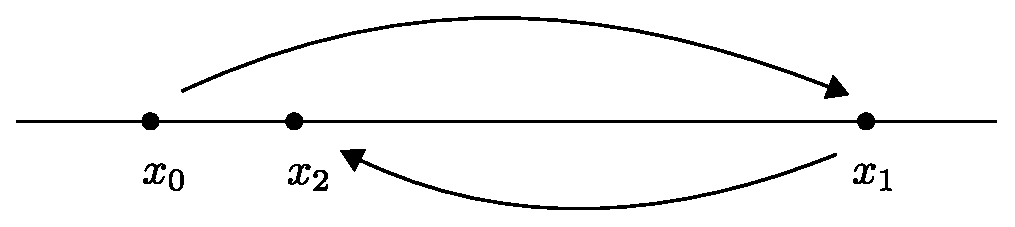
\includegraphics[width=0.7\textwidth]{F0_mapdiagram}
            \label{fig:F0_mapdiagram}
        \end{figure}

        Si el parámetro $A > 1$ el sistema presenta un crecimiento exponencial mientras que si $0 < A < 1$ presenta un decaimiento exponencial. Para toda condición inicial $x_{0}$ el sistema es atraído al punto $x = 0$ si $0 < A < 1$ y es atraído hacia el infinito si $A > 1$. Los sistemas cuya solución es atraída hacia el infinito son conocidos no acotado. El termino $A$ es un parámetro de control que rige la naturaleza de la dinámica. El valor $A = 1$ separa dos regiones en las que el comportamiento difiere y se denomina punto de bifurcación. Si $|A| < 1$ el sistema oscila alrededor de $x = 0$ y su amplitud decrece con el tiempo. Por lo tanto $x = 0$ es un atractor para toda $x_{0}$ cuando $|A| < 1$. Sin embargo cuando $A< -1$ crece exponencialmente hacia el infinito.

        Como el crecimiento exponencial no puede continuar para siempre, la ecuación (\ref{eq:crecimiento_exponencial}) es poco realista para cualquier proceso natural. Típicamente, alguna no linealidad detiene e incluso revierte el crecimiento. La no linealidad es despreciable en pequeños valores de $x$ pero empieza a dominar mientras más crece $x$. Una estrategia comúnmente utilizada es analizar primero el comportamiento lineal antes de introducir no linealidades. A pesar de que el sistema lineal pueda presentar deficiencias notorias, es importante comprender sus propiedades. 

        Imaginemos un cultivo de bacterias que crece cada hora, con las condiciones ideales de crecimiento la población aumenta sin restricciones y podemos modelar este comportamiento con la ecuación (\ref{eq:crecimiento_exponencial}). No obstante, si el espacio o el alimento escasea la población de bacterias no puede continuar creciendo a este ritmo. A medida que aumenta la población, el alimento y algunas bacterias mueren antes de poder dividirse. 

        Para incluir un término que reduzca el crecimiento a medida que $x$ aumenta es necesario modificar la ecuación (\ref{eq:crecimiento_exponencial}). La manera más sencilla es considerado que la tasa de crecimiento decrece linealmente, de manera que a la ecuación (\ref{eq:ecuacion_logistica}) se le conoce como ecuación logística.
            
       \begin{equation}
            x_{n+1} = A x_{n} (1 - x_{n}) 
            \label{eq:ecuacion_logistica}
       \end{equation}

       La no linealidad es cuadrática, debido a que el modelo se puede reescribir como $x_{n+1} = A x_{n} - A x_{n}^{2}$. El término cuadrático da una retroalimentación negativa no lineal y limita el crecimiento. La Figura \ref{fig:F1_logistic_curve} muestra la gráfica de la ecuación (\ref{eq:ecuacion_logistica}) con $A = 4$ llamada función logística o curva logística, la cual es una parábola.


        \begin{figure}[hbtp]
            \caption{El mapa logístico con $A = 4$.}
            \centering
            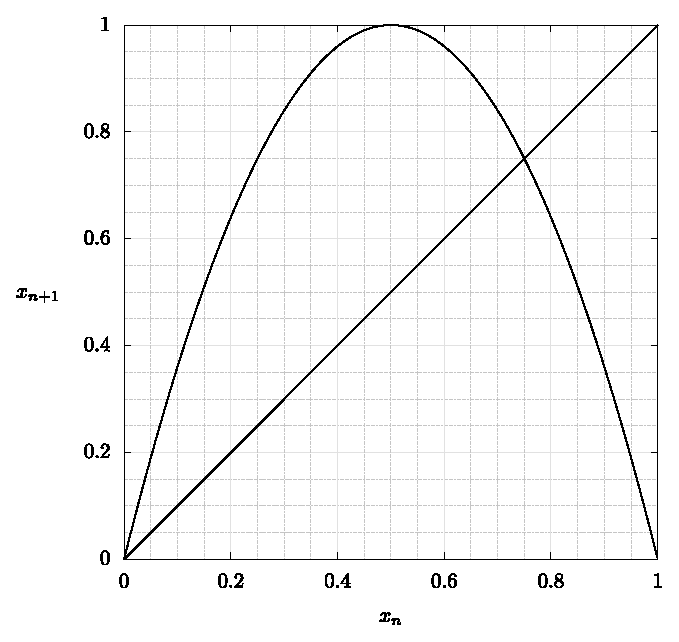
\includegraphics[width=0.6\textwidth]{F1_logistic_curve}
            \label{fig:F1_logistic_curve}
        \end{figure}

        En la Figura \ref{fig:F0_mapdiagram} también se muestra una recta descrita por $x_{n+1} = x_{n}$, a $45^{\circ}$ cuyas intersecciones con la parábola dan los valores de $x$ que no cambian con el tiempo. Para un mapa cuadrático, hay dos intersecciones de este tipo, que corresponden a las soluciones de la ecuación cuadrática que resultan de establecer $x_{n+1} = x_{n} = x^{*}$. Las soluciones $x^{*} = 0$ y $x^{*} = 1 - 1/A$ son llamados puntos fijos del mapa.

        Es interesante examinar cómo $x$ se aproxima a un punto fijo partiendo de una condición inicial $x_{o} \neq x^{*}$, esto lo hacemos con un diagrama de cobwebs. Los diagramas de cobwebs son una herramienta valiosa que nos permiten observar el comportamiento global de un sistema de manera intuitiva, proporcionando información complementaria a la obtenida mediante el análisis lineal. Son especialmente útiles resultan cuando el análisis lineal no es suficiente.

        Para construir el diagrama de cobwebs de un mapa iterado realizamos los siguientes pasos:

        Dado $x_{n+1} = f(x_{n})$ y una condición inicial $x_{0}$, trazar una línea vertical hasta que intersecte la gráfica $f$, esa altura es la salida $x_{1}$, en otras palabras dibujar una línea vertical desde $(x_{0}, 0) $ hasta $(x_{0}, x_{1})$. Después trazar una horizontal hasta intersectar con la linea diagonal $x_{n+1} = x_{n}$, es decir, dibujar una línea desde  $(x_{0}, x_{1}) $ hasta $(x_{1}, x_{1})$. Después trazar otra línea vertical hasta que intersecte la gráfica $f$ otra vez, una línea desde $(x_{1}, x_{1}) $ hasta $(x_{1}, x_{2})$. Repetir este proceso $n$ veces para generar los primeros $n$ puntos en la órbita.

        \begin{figure}[hbtp]
            \caption{Diagrama de cobwebs de mapa logístico con $A = 2.8$ y $x_{0} = 0.2$.}
            \centering
            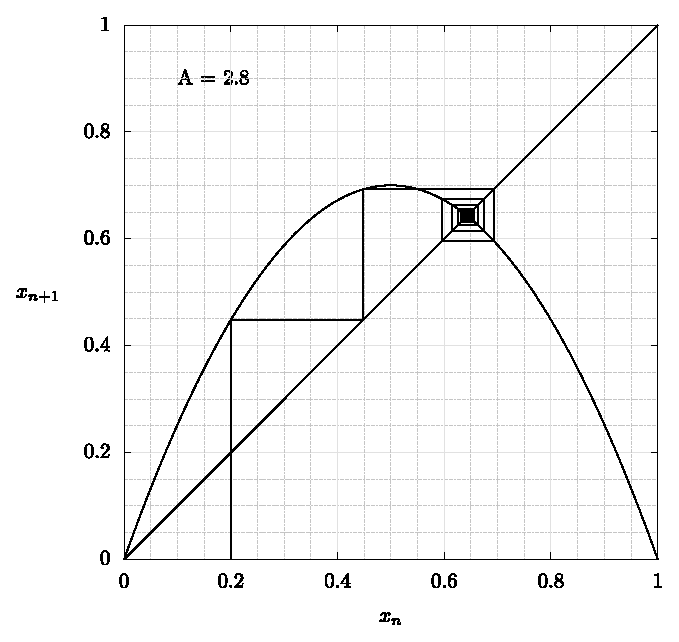
\includegraphics[width=0.6\textwidth]{F2_cobwebs_simple}
            \label{fig:F2_cobwebs_simple}
        \end{figure}

        Para el mapa logístico con $1 < A < 3,$ todos los puntos inicales en el intervalo $0 < x_{0} < 1$ se aproximan al punto fijo $x^{*} = 1 - 1/ A $, aunque la solución puede oscilar a su alrededor antes de llegar al valor final. El comportamiento recuerda al de un péndulo simple que oscila alrededor de la vertical antes de que la fricción lo lleve a reposar en su posición final. Otra manera de visualizar este comportamiento es gráficas la serie de tiempo, $x_{n}$ contra $n$, como se ve en la Figura \ref{fig:F3_time_series}. Es importante hacer la aclaración que se dibujaron lineas entre cada iteración para una mejor visualización, pero los datos son discretos. 

        \begin{figure}[hbtp]
            \caption{Serie de tiempo de mapa logístico con $A = 2.8$.}
            \centering
            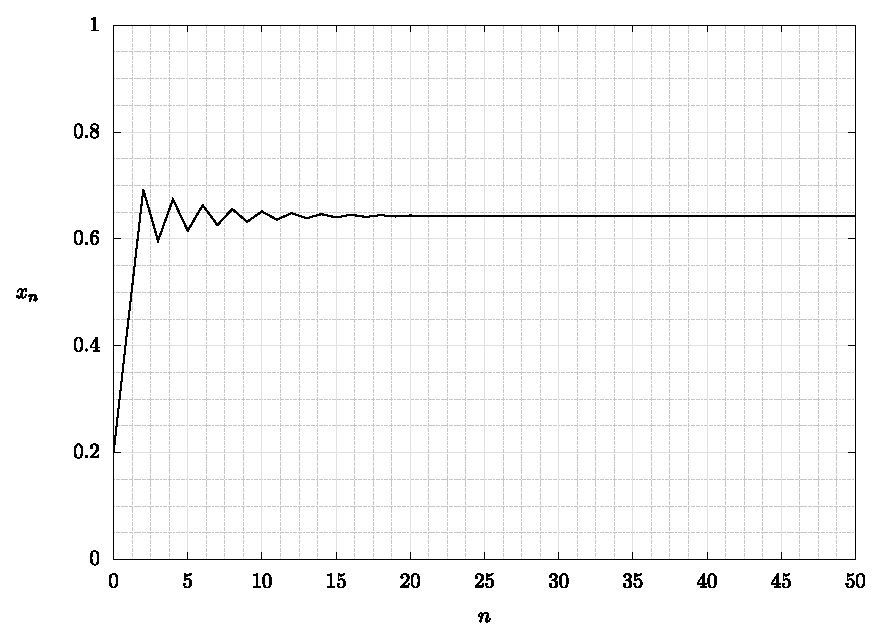
\includegraphics[width=0.6\textwidth]{F3_time_series}
            \label{fig:F3_time_series}
        \end{figure}

        En la ecuación de crecimiento exponencial en tiempo discreto (\ref{eq:crecimiento_exponencial}) cuando $A = \pm 1$ el comportamiento cambia abruptamente de acotado a no acotado. La ecuación logística se comporta de manera simular, excepto que hay más bifurcaciones y el comportamiento en varias regiones es más diverso e interesante. Es útil estudiar las bifurcaciones del mapa logístico porque las características generales son comunes a muchos sistemas caóticos. Consideraremos sólo valores positivos de $A$ y $x$.

        \begin{itemize}
            \item Caso $0 < A < 1$.
                En este rango la parábola solo puede intersectar a la linea de $45^{\circ}$ una vez en valores no negativos, y por lo tanto solo hay un punto fijo en $x^{*} = 0$. Todas las condiciones iniciales en el rango $0 < x_{o} < 1$ son atraídos hacia el punto $x^{*} = 0$. Decimos que estos puntos se encuentran dentro de una cuenca de atracción de $x_{0}$ y que el punto fijo $x_{0}$ es estable. Todos los puntos dentro de la cuenca de atracción se acercan al punto fijo con cada iteración. La no linealidad tiene poco efecto después de las primeras iteraciones. Los valores de $x_{0}$ fuera de de la cuenca de atracción están no acotados, escapan al infinito.
            \item Caso $1 < A < 3$.
                Al igual que con la ecuación (\ref{eq:crecimiento_exponencial}), para A = 1 se produce una bifurcación y el punto fijo en $x^{*} = 0$ se vuelve inestable. El atractor se convierte en un repulsor. Si $x$ resulta ser exactamente cero, permanecerá así, pero si es incluso ligeramente positivo, crecerá inicialmente a un ritmo exponencial. La situación es como la de un lápiz apoyado sobre su extremo puntiagudo. El más mínimo empujón hará que se caiga. Sin embargo, a diferencia de la ecuación (\ref{eq:crecimiento_exponencial}) en la que las soluciones son ilimitadas, el mapa logístico en $A = 1 $ desarrolla un nuevo punto fijo en $x^{*} = 1- 1/A = 0$ que se aleja de cero para $A > 1$. Si $A$ no es demasiado grande, entonces ese punto es un atractor porque todos los valores iniciales en el rango $0 < x_{0} < 1$ son atraídos hacia él y finalmente se asientan en él. Decimos que el estado final es un ciclo de periodo 1, o simplemente un ciclo de 1, porque cada iteración es la misma que la anterior. Si la ecuación logística estuviera modelando la población de bacterias, entonces predeciría un crecimiento exponencial inicial para este rango de $A$, pero un estado estacionario final en el que el número de bacterias no cambia.
            \item Caso $3 < A < 3.44948$.
                Para $A = 3$, el punto fijo en $x^{*} = 1 - 1/A$ sigue existiendo, pero cambia de estable a inestable, convirtiéndose en un repulsor. Esta bifurcación se produce cuando la pendiente de la parábola en el punto fijo es igual a $-1$. Para $A > 3$ tenemos un crecimiento exponencial alejándonos del punto, en lugar de una caída exponencial hacia él. Como la pendiente es negativa, la solución oscila a ambos lados del punto fijo mientras se aleja, igual que en la ecuación (\ref{eq:crecimiento_exponencial}) con $ A < -1$. De ahí que la bifurcación en $A = 3$ se denomine flip. Sin embargo, el crecimiento no continúa para siempre. En su lugar, se acerca a una condición en la que cada iterado es el mismo $x_{n} = x_{n+2} = x_{n+4}$ como en el diagrama de cobwebs de la Figura \ref{fig:F5_cobwebs_bifurcation} Con un poco de álgebra, esta condición puede reducirse a una ecuación de cuarto grado.

                \begin{equation}
                    A^{3} x^{4} - 2 A^{3} x^{3} + A^{2} (A + 1) x^{2} - (A^{2} -1)x = 0
                \end{equation}

                Como cualquier ecuación cuadrática, tiene cuatro raíces. 


                


        \begin{figure}[hbtp]
            \caption{Diagrama de cobwebs de mapa logístico con $A = 3.2$ y $x_{0} = 0.1$.}
            \centering
            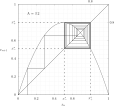
\includegraphics[width=0.6\textwidth]{F5_cobwebs_bifurcation}
            \label{fig:F5_cobwebs_bifurcation}
        \end{figure}


        \begin{figure}[hbtp]
            \caption{Diagrama de bifurcación de mapa logístico.}
            \centering
            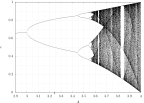
\includegraphics[width=0.6\textwidth]{F4_bifurcation}
            \label{fig:F4_bifurcation}
        \end{figure}


        \end{itemize}

    \section{Análisis de mapa logístico}

        Consideremos la ecuación $x_{n+1} = A x_{n} (1 - x_{n})$ para $0 \leq x_{n} \leq 1$ y $0 \leq A \leq 4$. Los puntos fijos satisfacen $x^{*} = f(x^{*}) = A x^{*}(1 - x^{*})$. Por lo tanto $x^{*} = 0$  o $x^{*} = 1 - 1/A$. El origen es un punto fijo para todas las $A$, mientras que $x^{*} = 1 - 1/A$ solo es valido para las $x \geq 1$. La estabilidad depende de $f'(x^{*}) = A - 2Ax^{*}$. Como $f'(0) = A $ el origen es estable para $A < 1$ e inestable para $A < 1$. En el otro punto fijo, $f'(x^{*}) = A - 2 A \left( 1 - \frac{1}{A} \right) = 2 - A$. Entonces $x^{*} 1 - \frac{1}{A} $ es estable para $1 < A < 3$.

    \section{Puntos fijos y estabilidad lineal}
        

            

Libro para el publico general \cite{Gleick1987}
 
